%% Bookheader, Nov 8, 2020; July 18, 2022

\documentclass[11pt]{../Support/ourbook}
%% or for landscape, comment out line above and use this one:
%%\documentclass[landscape,11pt]{ourbook}

%% This will keep space from stretching around display math:

\makeatletter
\renewcommand\normalsize{%
   \@setfontsize\normalsize\@xipt{13.6}%
   \abovedisplayskip 11\p@  \@minus6\p@
   \abovedisplayshortskip \z@ 
   \belowdisplayshortskip 6.5\p@ \@minus3\p@
   \belowdisplayskip \abovedisplayskip
   \let\@listi\@listI}
\makeatother
\normalsize


\begin{document}

\tableofcontents
\graphicspath{{../../Chapters/projections/en_US}}
\chapter{Projections}

The word projection has two main meanings in everyday life. One is a projection as a forecast or estimate of something in the future based on the current situation. Another is the result of shining a light to cast a shadow or show a movie. Both these definitions apply to mathematical projection.

Projections are used in many fields such as science, math, engineering, and finance. Here are a few examples: 
\begin{itemize}
\item Investors evaluate risk and return of a portfolio by projecting an asset’s return onto a reference portfolio.
\item Astronomers analyze the motion of stellar objects by projecting the object’s true motion onto the plane of the sky.
\item Robotics engineers use projections to prevent robots from running into obstacles by projecting the robot’s position onto the optimal path.
\end{itemize}

Mathematically, a projection describes the relationship of one vector to another in terms of direction and orthogonality. Given two vectors, $\mathbf{u}$ and $\mathbf{v}$, the projection of $\mathbf{u}$ onto $\mathbf{v}$ separates $\mathbf{u}$ into two components. The first component signifies how much $\mathbf{u}$ lies in the direction of $\mathbf{v}$. The second signifies the component of $\mathbf{u}$ that is orthogonal (perpendicular) to $\mathbf{v}$. \index{projection} 

The figure depicts a projection. The perpendicular line dropped from the end of $\mathbf{u}$ is the orthogonal component. The portion of $\mathbf{u}$ that lies in the direction of $\mathbf{v}$ is the blue segment. 

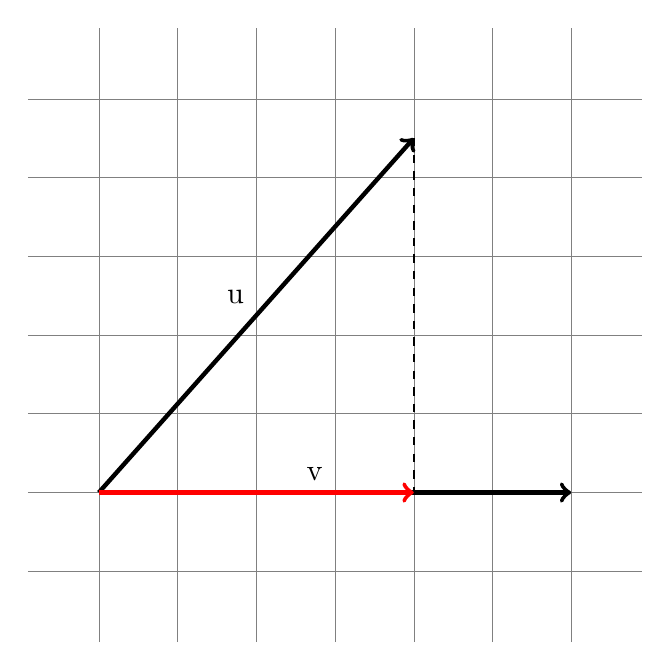
\begin{tikzpicture}
\draw[step=1cm, gray, very thin](-1.9, -1.9) grid (5.9,5.9);
\draw[black, ultra thick, ->] (-1,0) -- (3,4.5) node[midway,above left] {u};
\draw[black, ultra thick, ->] (-1,0) -- (5,0) node[midway,above left] {v};
\draw[black, thick, dashed] (3,4.5) -- (3,0);
\draw[red, ultra thick, ->] (-1,0) -- (3,0);
\end{tikzpicture}

You can also think of a projection as the shadow cast by one vector onto each other by an overhead light.

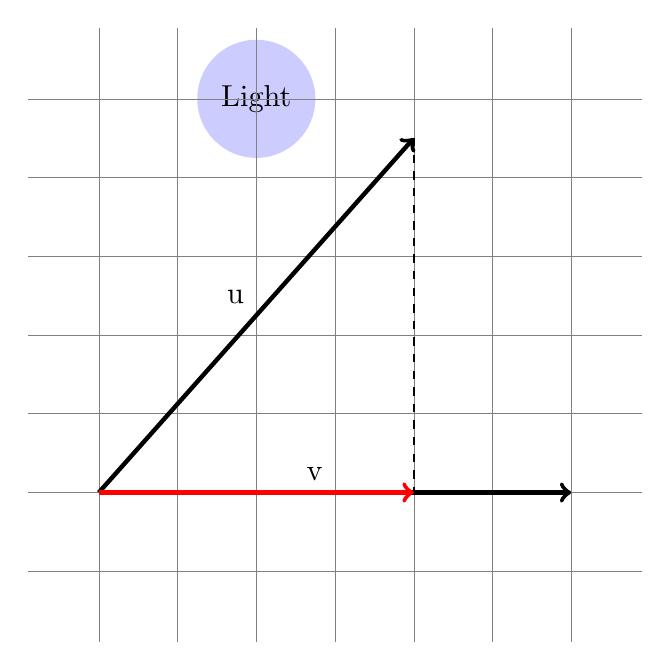
\begin{tikzpicture}[fatnode/.style={circle, fill=blue!20, minimum size=15mm}]
\node[fatnode] (A) at (1, 5) {Light};
\draw[step=1cm, gray, very thin](-1.9, -1.9) grid (5.9,5.9);
\draw[black, ultra thick, ->] (-1,0) -- (3,4.5) node[midway,above left] {u};
\draw[black, ultra thick, ->] (-1,0) -- (5,0) node[midway,above left] {v};
\draw[black, thick, dashed] (3,4.5) -- (3,0);
\draw[red, ultra thick, ->] (-1,0) -- (3,0);
\end{tikzpicture}

The projected vector can be in any direction and its length can extend beyond the vector onto which it is projecting.

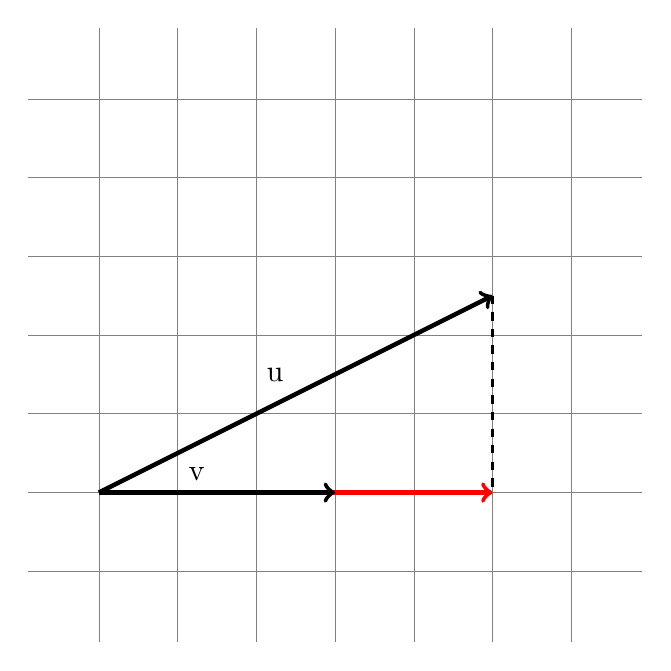
\begin{tikzpicture}  
\draw[step=1cm, gray, very thin](-1.9, -1.9) grid (5.9,5.9);
\draw[black, ultra thick, ->] (-1,0) -- (4,2.5)node[midway,above left] {u};
\draw[red, ultra thick, ->] (-1,0) -- (4,0);
\draw[black, ultra thick, ->] (-1,0) -- (2,0)node[midway,above left] {v};
\draw[black, thick, dashed] (4,2.5) -- (4,0);
\end{tikzpicture}

To calculate the projection of 
$\mathbf{v}$ onto $\mathbf{u}$,use this formula:

$$\mathbf{proj}_\mathbf{v}(\mathbf{u}) = \frac{u\cdot v}{\parallel{v}\parallel ^2}v$$

Note that the denominator is is the magnitude squared of vector $\mathbf{v}$.
$$(\sqrt{a_1^2 + a_2^2 + ... + a_n^2} )^2$$
You learned previously that this is the same as the dot product of a vector with itself.
$${v\cdot v}$$
In the examples that follow, we'll simplify to the dot product notation.

Let's look at a specific example:
$$u = (1,4,6)$$ 
$$v = (-2,6,2)$$ 

$$\mathbf{proj}_\mathbf{v}(\mathbf{u}) = \frac{u\cdot v}{\parallel {v}\parallel ^2}v$$
$$\mathbf{proj}_\mathbf{v}(\mathbf{u}) = \frac{(1,4,6)\cdot(-2,6,2)}{ (-2,6,2)\cdot (-2,6,2)}(-2,6,2)$$
$$\mathbf{proj}_\mathbf{v}(\mathbf{u}) = (\frac{34}{44}(-2,6,2)$$
$$\mathbf{proj}_\mathbf{v}(\mathbf{u}) = (-1.545, 4.64, 1.545)$$

As you work your way through this course, you'll have a chance to apply the calculations you learn in this chapter to a variety of problems. Specifically, the next chapter shows how to transform a set of linearly independent vectors into a set of orthogonal ones. Projections are essential to that transformation. 

\begin{Exercise}[title={Projections}, label=projections]
	Find the projection of $\mathbf{a}$ on $\mathbf{b}$ where:
	$$a = (1,3)$$
	$$b = (-4,6)$$
\end{Exercise}
\begin{Answer}[ref=project_vector]
	Compute dot product of $\mathbf{a}$ and $\mathbf{b}$:
	$$1*-4 + 3*6 = -4 +18 = 14$$
	Compute the dot product of $\mathbf{b}$ and $\mathbf{b}$
	$$16 + 36 = 52 $$
	$$14/52 * (-4,6) = (-1.076 , 1.61)$$
\end{Answer}
 
\section{Projections in Python}

Create a file called \filename{vectors\_projections.py} and enter this code:
\begin{Verbatim}
import numpy as np

# define two vectors  
a = np.array([1, 4, 6])   
b = np.array([-2, 6, 2])  
  
# use np.dot() to calculate the dot product
projection_a_on_b = (np.dot(a, b)/np.dot(b, b))*b
  
print("The projection of vector a on vector b is:", projection_a_on_b)
\end{Verbatim}
 
\section{Where to Learn More}

Watch this Introduction to Projections from Khan Academy 
\url{https://rb.gy/yf0i3}


\graphicspath{{../../Chapters/gram-schmidt/en_US}}
\chapter{The Gram-Schmidt Process}

The Gram-Schmidt process is a method use to transform a set of linearly independent vectors to a set of orthogonal (perpendicular vectors). The original vectors and the transformed vectors span the same subspace. 

The process was named after two mathematicians: Jørgen Pedersen Gram, a Danish actuary mathematician, and Erhard Schmidt, a German mathematician. The men developed the orthogonalization process independently. Gram introduced the process in 1883 whereas Schmidt did his work in 1907.  It wasn’t named the Gram-Schmidt process until sometime later, after both mathematicians became well-known in the mathematical community.

In the last chapter you learned how to calculate a projection of one vector on another. Given two vectors, $u$ and $v$, the projection separates $u$ into the part that is orthogonal to $v$ and the part that has a dependency with $v$. The Gram-Schmidt process builds on the notion of projections to iteritively strip away dependencies between vectors until the vectors that remain are orthogonal. If there happens to be a vector that is a linear combination of the others, that vector will be reduced to the zero vector. The vectors that remain define a new basis for space spanned by the original set of vectors. 

Gram-Schmidt has many practical applications in science and engineering. These are two examples:
\begin{enumerate}
\item In signal processing, it can represent an audio signal with fewer components making it easier to isolate and remove noise. 
\item In statistics and data analysis, it can reduce the complexity of a dataset so that it is easier to see which aspects or features contribute to the analysis. 
\end{enumerate}

\section{The Process}

The Gram-Schmidt process orthonormalizes a set of vectors in an inner product space, most commonly the Euclidean space
$\mathbb{R}^n$. The process takes a finite, linearly independent set
$S = \{v_1, v_2, \ldots, v_k\}$ for $k \leq n$, and generates an
orthogonal set $S' = \{u_1, u_2, \ldots, u_k\}$ that spans the same
k-dimensional subspace of $\mathbb{R}^n$ as $S$.\index{Gram-Schmidt process}

Let's look at how the process works. Given a set of vectors $S = \{v_1, v_2, \ldots, v_k\}$, the Gram-Schmidt process is as follows:

\begin{enumerate}
    \item Let $u_1 = v_1$.
    \item For $j = 2, 3, \ldots, k$:
    \begin{enumerate}
        \item Let $w_j = v_j - \sum_{i=1}^{j-1} \frac{\langle v_j, u_i \rangle}{\langle u_i, u_i \rangle} u_i$
        \item Let $u_j = w_j$
    \end{enumerate}
\end{enumerate}

Here, $\langle . , . \rangle$ denotes the inner product. 

The set of vectors $S' = \{u_1, u_2, \ldots, u_k\}$ obtained from this
process is orthogonal, but not necessarily orthonormal. To create
an orthonormal set, you simply need to normalize each vector $u_i$ to
unit length. That is, $u_i' = \frac{u_i}{\|u_i\|}$, where $\|.\|$
denotes the norm (or length) of a vector.

Among other things, making vectors orthonormal simplifies calculations, makes it easier to define rotations and transformations, and provides a framework for calculations in fields such as quantum mechanics.

\section{Example Calculation}

Given a set of linearly independent vectors, we will use the Gram-Schmidt process to find an orthogonal basis.

Let $$W = Span (x_1, x_2, x_3)$$ where
$$x_1 = (1, 2, -2) $$
$$x_2 = (1,0,-4) $$
$$x_3 = (5,2,0)$$

The three orthogonal vectors will define the same subspace as the original vectors. 

The first vector of the orthogonal subspace is easy to define. We set it to be the same as $x_1$.

$$v_1 = x_1 = (1, 2, -2)$$

The second orthogonal vector is a projection of $x_2$ onto $v_1$. You learned projections in the last chapter, so this should be fairly straightforward.

$$v_2 = x_2 - \frac{x_2v_1}{v_1v_1} v_1$$

Substitute the values:

$$v_2 = (1, 0, -4)  - \frac{(1,0, -4)(1,2,-2)}{(1,2,-2)(1,2,-2)} \ (1, 2, -2) $$

Calculate the coefficient for $v_1$:
$$v_2 = (1, 0, -4) - \frac{9}{9} (1, 2, -2)  \\$$
Perform the subtraction:
$$v_2 = (0, -2, -2) \\$$
 
The third vector for the orthogonal subspace is a projection onto $v_1$ and $v_2$. 
$$v_3 = x_3 - \frac{x_3v_1}{v_1v_1} v_1 - \frac{x_3v_2}{v_2v_2} v_2$$

Substitute the values:
$$v_3 = (5,2,0) - \frac{(5,2,0)(1,2,-2)}{(1,2,-2)(1,2,-2)} (1,2,-2) - \frac{(5,2,0)(1,0,-4)}{(1,0,-4)(1,0,-4)} (1,0,-4)$$
$$v_3 =  (5,2,0)  - (9/9) (1,2,-2) -  (-4/8)(1,0,-4)$$
$$v_3 =  (5,2,0) - (1,2,-2) + (1/2)(1,0,-4)$$
$$v_3  = (5,2,0 ) - (1,2,-2) + (0,-1,-1)$$
$$v_3 = (4, -1, 1)$$

This set of vectors is orthogonal, so we need to normalize them so that the vectors are orthonormal. Recall that an orthonormal vector has a length of 1 and is computed using this formula:
$$normalizedVector = vector / np.sqrt(np.sum(vector**2))$$
Thus the normalized set of vectors is:
$$v_1 = (0.33,  0.67, -0.67)$$
$$v_2 = (0.0,  -0.71, -0.71 )$$
$$v_3 = (0.94, -0.24,  0.24 ) $$

\begin{Exercise}[title={Gram-Schmidt Process}, label=gram_schmidt]
    Use the Gram-Schmidt process to to find an orthogonal basis for the span defined by $x_1, x_2$ where:
    $$x_1 = (1, 1, 1)$$
	$$x_2 = (0, 1, 1) $$
\end{Exercise}
\begin{Answer}[ref=gram_schmidt]
      The first vector of the orthogonal subspace is: 
		$$v_1 = x_1 =  (1, 1, 1) $$ 
	  The second vector of the subspace is a projection of $x_2$ onto $v_1$.
	  $$v_2 = x_2 - \frac{x_2v_1}{v_1v_1} v_1$$
	  Substitute the values:
	  $$v_2 =  (0, 1, 1)  - \frac{(0,1, 1)(1,1,1)}{(1,1,1)(1,1,-1)}  (1, 1, 1)$$
	  $$v_2 =  (0, 1, 1)  - (2/3) (1, 1, 1) $$
	  $$v_2 =  (-2/3, 1/3, 1/3)$$
	  Normalize:
	  $$v_1 = v_1/\sqrt{|v_1|} $$
	  $$v_1 = (1, 1, 1 )/\sqrt{|v_1|} $$
	  $$v_1 = (0.577, 0.577, 0.577)  $$  
	  $$v_2 = v_2/\sqrt{|v_2|} $$
	  $$v_2 = (0, 1, 1) \sqrt{|v_2|} $$
	  $$v_2 =  (-0.816,  0.408,  0.408) $$
\end{Answer}

\section{The Gram-Schmidt Process in Python}
Create a file called \filename{vectors\_gram-schmidt.py} and enter this code:
\begin{Verbatim}
# import numpy to perform operations on vector
import numpy as np

# Find an orthogonal basis for the span of these three vectors  
x1 = np.array([1, 2, -2]) 
x2 = np.array([1, 0, -4]) 
x3 = np.array([5, 2, 0])    
   
# v1 = x1
v1 = x1
print("v1 = ",v1)

# v2 = x2 - (the projection of x2 on v1)
v2 = x2 - (np.dot(x2,v1)/np.dot(v1,v1))*v1
print("v2 = ", v2)

# v3 = x3 - (the projection of x3 on v1) - (the projection of x3 on v3)
v3 = x3 - (np.dot(x3,v1)/np.dot(v1,v1))*v1 - (np.dot(x3,v2)/np.dot(v2,v2))*v2
print("v3 =", v3)

# Next, normalize each vector to get a set of vectors that is both orthogonal and orthonormal:
v1_norm = v1 / np.sqrt(np.sum(v1**2))
v2_norm = v2 / np.sqrt(np.sum(v2**2))
v3_norm = v3 / np.sqrt(np.sum(v3**2))
print("v1_norm = ", v1_norm)
print("v2_norm = ", v2_norm)
print("v3_norm = ", v3_norm)
\end{Verbatim}

\section{Where to Learn More}
Watch this video from Khan Academy about the Gram-Schmidt process: \url{https://www.khanacademy.org/math/linear-algebra/alternate-bases/orthonormal-basis/v/linear-algebra-the-gram-schmidt-process}

\graphicspath{{../../Chapters/eigen/en_US}}
\chapter{Eigenvectors and Eigenvalues}


Like many specialized disciplines, Linear Algebra uses many unfamiliar terms whose origin you might wonder about. Eigenvectors and eigenvalues are two of them. If you know German, you’ll recognize that eigen means inherent or a characteristic attribute. Named by the German mathematician David Hilbert, an eigenvector mathematically describes a characteristic feature of an object, that remains unchanged after transformation. You can think of an eigenvector as the direction that doesn’t change direction. 

Eigenvalues and eigenvectors are a way to break down matrices that can simplify many calculations and enable us to understand various properties of the matrix. They are widely used in physics and engineering for stability analysis, vibration analysis, and many other applications. \index{eigenvector} \index{eigenvalue}

Let’s look at a visual example.

\includegraphics[width=0.8\textwidth]{eigensquirrel.png}

You can see that the  image on the right is a skewed version of the image on the left. Look closely at the vectors and you’ll notice that the one of the vectors is pointing in the same direction in both images, while the direction of the other two vectors has changed. The eigenvector is the one at the bottom that points 0 degrees (or you can think of due east) in both images. Thus the characteristic attribute of both images is their horizontal direction.

When you overlay the vectors from one image over the other, you’ll notice that the horizontal vector, while the same direction in both images, is a bit longer in the skewed version. The scale of the stretch is described by an eigenvalue.

\includegraphics[width=0.4\textwidth]{overlaysquirrel.png}


\section{Definition}

Given a square matrix $A$, a non-zero vector $v$ is an eigenvector of
$A$ if multiplying $A$ by $v$ results in a scalar multiple of $v$,
i.e.,

\begin{equation}
Av = \lambda v
\end{equation}

where $\lambda$ is a scalar known as the eigenvalue corresponding to the eigenvector $v$.

\section{Finding Eigenvalues and Eigenvectors}

You find the eigenvalues of a matrix $A$  by solving the characteristic equation:

\begin{equation}
\text{det}(A - \lambda I) = 0
\end{equation}

where $\text{det}(.)$ denotes the determinant, $I$ is the identity
matrix of the same size as $A$, and $\lambda$ is a scalar.

Once your find the eigenvalues, you can find the corresponding eigenvectors by substituting each eigenvalue into the equation $Av = \lambda
v$, and solving for $v$.

\section{Example}

For a $2 \times 2$ matrix $A = \begin{pmatrix} a & b \\ c &
  d \end{pmatrix}$, the characteristic equation is:

\begin{equation}
(a - \lambda)(d - \lambda) - bc = 0
\end{equation}

Solving this equation  gives the eigenvalues. Substituting each
eigenvalue back into the equation $Av = \lambda v$ gives the
corresponding eigenvectors.

Let matrix $A$ =
$$\begin{bmatrix}
5,4 &\\
 1,2& 
\end{bmatrix} $$

The characteristic equation is: 
$$|A - \lambda I| = 0$$ 
$$\begin{bmatrix}
5 - \lambda,4 &\\
 1,2- \lambda& 
\end{bmatrix} = 0$$
$$(5 - \lambda) (2 - \lambda) - (4)(1) = 0$$
$$10 - 5\lambda - 2\lambda + \lambda2 - 4 = 0$$
$$\lambda2 - 7\lambda + 6 = 0$$
$$(\lambda - 6)(\lambda - 1) = 0$$
$$\lambda = 6, \lambda = 1$$
Now that you have the eigen values you can substitue these values into the equation: 
$$|A - \lambda I| = 0$$ 
For $λ = 1$:
$$(A - \lambda I) v = O$$
$$\begin{bmatrix}
5-1, 4 &  \\
 1, 2-1& 
\end{bmatrix}
\begin{bmatrix}
x&  \\
 y& 
\end{bmatrix} = 
\begin{bmatrix}
0&  \\
0& 
\end{bmatrix}$$
$$\begin{bmatrix}
4, 4 &  \\
 1, 1& 
\end{bmatrix}
\begin{bmatrix}
x&  \\
 y& 
\end{bmatrix} = 
\begin{bmatrix}
0&  \\
0& 
\end{bmatrix}$$
Next,use elementary row transformation by multiplying row 2 by 4 and then subtracting row 1.
$$\begin{bmatrix}
4, 4 &  \\
 0, 0& 
\end{bmatrix}
\begin{bmatrix}
x&  \\
 y& 
\end{bmatrix} = 
\begin{bmatrix}
0&  \\
0& 
\end{bmatrix}$$
Now you can expand as an equation:
$$4x + 4y = 0$$
Assume y = w
$$4x = -4w$$
$$x = -w$$
The solution is:
$$\begin{bmatrix}
x&  \\
y& 
\end{bmatrix} = 
\begin{bmatrix}
-w&  \\
w& 
\end{bmatrix} = 
w\begin{bmatrix}
-1&  \\
1&
\end{bmatrix}$$
So the eigenvector is:
$$\begin{bmatrix}
-1&  \\
1&
\end{bmatrix}$$
Now we need to substitue the other eigenvalue, 6, into the equation and follow the same procedure for finding the eigenvector. 
$$\begin{bmatrix}
5-6, 4 &  \\
 1, 2-6& 
\end{bmatrix}
\begin{bmatrix}
x&  \\
 y& 
\end{bmatrix} = 
\begin{bmatrix}
0&  \\
0& 
\end{bmatrix}$$
$$\begin{bmatrix}
-1, 4 &  \\
 1, -4& 
\end{bmatrix}
\begin{bmatrix}
x&  \\
 y& 
\end{bmatrix} = 
\begin{bmatrix}
0&  \\
0& 
\end{bmatrix}$$
Next, use elementary row transformation by adding row 1 to row 2.
$$\begin{bmatrix}
-1, 4 &  \\
 0, 0& 
\end{bmatrix}
\begin{bmatrix}
x&  \\
 y& 
\end{bmatrix} = 
\begin{bmatrix}
0&  \\
0& 
\end{bmatrix}$$
Expand as an equation:
$$-x + 4y = 0$$
Assume y = w
$$-x + 4w = 0$$
$$x = 4w$$
The solution is:
$$\begin{bmatrix}
x&  \\
y& 
\end{bmatrix}=
\begin{bmatrix}
4w&  \\
w& 
\end{bmatrix} =
w\begin{bmatrix}
4&  \\
1& 
\end{bmatrix}$$
So the eigenvector is:
$$\begin{bmatrix}
4&  \\
1&
\end{bmatrix}$$
In conclusion, the eigenvectors of the given 2 x 2 matrix are:
$$\begin{bmatrix}
-1&  \\
1&
\end{bmatrix}
and \begin{bmatrix}
4&  \\
1&
\end{bmatrix}$$

\section{Eigenvalues and Eigenvectors in Python}
Create a file called \filename{vectors\_eigen.py} and enter this code:

\begin{Verbatim}
# import numpy to perform operations on vector
import numpy as np
from numpy.linalg import eig

a = np.array([[2, 2, 4], 
              [1, 3, 5],
              [2, 3, 4]])
eigenvalue,eigenvector = eig(a)

# The values are not in any particular order
print('Eigenvalues:', eigenvalue)

# The eig function returns the normalize vectors
print('Eigenvectors:', eigenvector)

\end{Verbatim}

\section{Where to Learn More}
Watch this video from Khan Academy, \emph{Introduction to Eigenvectors}: \url{https://rb.gy/mse7i}

\graphicspath{{../../Chapters/decomposition/en_US}}
\chapter{Singular Value Decomposition}

In the previous chapter you learned how to calculate eigenvalues and eigenvectors. But not every matrix has them. For those matrices, singular values and singular vectors are analogous features. 

Singular Value Decomposition (SVD) is a matrix factorization technique that breaks down a matrix into three matrices that represent the structure and properties of the original matrix.The decomposed matrices make calculations easier and provide insight into the original matrix. Basically, SVD can transform a high dimension, highly variable set of data into a set of uncorrelated data points that reveal subgroupings that you might not have noticed in the original data.
\index{singular value decomposition} \index{svd}


\section{Definition}

For any $m \times n$ matrix $A$, decomposes the matrix into three matrices.

\begin{equation}
A = U \Sigma V^T
\end{equation}

$U$ and $V$ are orthogonal matrices. \Sigma is a diagonal matrix that is the same size as $A$. Its diagonal contain the singular values of $A$. 

\begin{itemize}
\item $U$ is an orthogonal matrix whose size is $m \times m$. Its columns are the
  eigenvectors of $AA^T$. These are the left singular vectors of $A$. Because $U$ is orthogonal,$U^TU = I$
\item $V$ is an orthogonal matrix whose size is $n \times n$ matrix. Its columns are the
  eigenvectors of $A^TA$. These are the right singular vectors of $A$. Because $V$ is orthogonal, $V^TV = I$.
\item  \Sigma is a diagonal matrix that is the same size as $A$. Its diagonal contains the singular values of $A$, arranged in descending order. These values are the square roots of the eigenvalues of both $A^TA$ and  $AA^T$. 
\end{itemize}

\section{Applications of SVD}

SVD has numerous applications:

\begin{itemize}
\item It's used in machine learning and data science to perform
  dimensionality reduction, particularly through a technique known as
  Principal Component Analysis (PCA).

\item In numerical linear algebra, SVD is used to solve linear
  equations and compute matrix inverses in a more numerically stable
  way.

\item It's used in image compression, where low-rank approximations of
  an image matrix provide a compressed version of the original image.
\end{itemize}

\section{Calculating SVD Manually}
You might be inclined to skip this example because the computations are lengthy. Why would anyone do this when they can use a computing language, like Python, to calculate the SVD with essentially one command? We show this so you can understand what goes on "under the hood" when you compute SVD programmatically. 

After you read through this example, you'll see how to use Python to compute SVD. Then you'll see an example of using SVD for image compression. Finally, you'll have an exercise to compute the SVD. For this, you'll need to write your own Python script.

Let's find the SVD for matrix $A$. Recall that we want to find $U$. $\Sigma$, and $V^T$ such that:

\begin{equation}
A = U \Sigma V^T
\end{equation}

$$ A = \begin{bmatrix}
3,1,1 &  \\
 -1, 3,1& 
\end{bmatrix}$$

$$U = AA^T$$ 

Start with $A^T$:
$$ A^T = \begin{bmatrix}
3,-1 &  \\
1,3 &  \\
1,1& 
\end{bmatrix}$$
$$AA^T = \begin{bmatrix}
3,1,1 &  \\
 -1, 3,1& 
\end{bmatrix}
\begin{bmatrix}
3,-1 &  \\
1,3 &  \\
1,1& 
\end{bmatrix}
= \begin{bmatrix}
11,1 &  \\
 1, 11& 
\end{bmatrix}
$$
Next we will find the eigenvalues and eigenvectors of $A^T$. This is a chance to apply what you learned in the previous chapter. We know that:
\begin{equation}
Av = \lambda v
\end{equation}
So:
$$
\begin{bmatrix}
11,1 &  \\
 1, 11& 
\end{bmatrix}
\begin{bmatrix}
x_1 &  \\
x_2& 
\end{bmatrix}
=
\lambda 
\begin{bmatrix}
x_1 &  \\
x_2& 
\end{bmatrix}
$$
Rewrite as a set of equations:
$$11x_1 + x_2 = \lambda x_1$$
$$x_1 + 11x_2 = \lambda x_2$$
Then rearrange:
$$(11−\lambda )x_1 +x_2 =0$$
$$x_1 +(11−\lambda )x_2 =0 $$
Solve for \lambda :
$$\begin{bmatrix}
(11 -\lambda), 1 \\
 1, (11 -\lambda) 
\end{bmatrix} = 0$$
And as equations:
$$(11 − \lambda)(11 − \lambda) − 1 · 1 = 0$$
$$(\lambda − 10)(\lambda − 12) = 0$$
These are the eigenvalues.
$$\lambda = 10$$
$$\lambda = 12$$
When substituted into the original equations, you get the eigenvectors. For $$ \lambda = 10$$:
$$(11−10)x_1 +x_2 =0 $$
$$x_1 = -x_2$$
We'll set $$x_1$$ to 1 and get this eigenvector:
$$\left[ 1,-1 \right]$$
For $$ \lambda = 10$$:
$$(11−12)x_1 +x_2 =0  $$
$$x_1 = x_2 $$
We'll set $$x_1$$ to 1 and get this eigenvector:
$$\left[ 1,1 \right]$$
The matrix is:
$$
\begin{bmatrix}
1,1 \\
1,-1 
\end{bmatrix}
$$
Next you need to apply the Gram-Schmidt process to the column vectors. Then you'll have $U$, the $m \times m$ matrix whose columns are eigenvectors of $AA^T$. These are the left singular vectors of $A$. After you apply Gram-Schmidt, you should end up with:
$$
U = \begin{bmatrix}
1/\sqrt{2},1/\sqrt{2} \\
1/\sqrt{2},-1/\sqrt{2} 
\end{bmatrix}
$$
The process for calculating $V$ is the same as the calculation for $U$, except:
$$V = A^TA$$ 
$$A^TA = 
\begin{bmatrix}
3,-1 &  \\
1,3 &  \\
1,1& 
\end{bmatrix}
\begin{bmatrix}
3,1,1 &  \\
 -1, 3,1& 
\end{bmatrix}
=
\begin{bmatrix}
10,0,2 \\
0,10,4 \\
 2,4,2
\end{bmatrix}
$$
After applying the process we applied to solve for U, you get:
$$
V = \begin{bmatrix}
1/\sqrt{6},2/\sqrt{5},1/\sqrt{30} \\
2/\sqrt{6},-1/\sqrt{5},2/\sqrt{30}\\
1/\sqrt{6},0,-5/\sqrt{30}
\end{bmatrix}
$$
However, you want $V_T$:
$$
V_T =
\begin{bmatrix}
1/\sqrt{6},2/\sqrt{6},1/\sqrt{6} \\
2/\sqrt{5},-1/\sqrt{5},0\\
1/\sqrt{30},2/\sqrt{30},-5/\sqrt{30}
\end{bmatrix}
$$
You have only to calculate $\Sigma$, a diagonal matrix that is the same size as $A$. The diagonal contains the singular values of $A$, arranged in descending order. They are the square roots of the eigenvalues of both $A^TA$ and  $AA^T$.

Because the non-zero eigenvalues of U are the same as V, let's use the eigenvalues we calculate for U, 10 and 12. Note that $\Sigma$ will not be of the correct dimension to reconstruct the orignal matrix unless we add a column. By adding a zero column you'll be able to multiply between $U$ and $V$:
$$
\Sigma = 
\begin{bmatrix}
\sqrt{12}, &0,&0\\
 0,&\sqrt{12}  &0 
\end{bmatrix}
$$
You can check your work by multiplying the decomposed matrices. This should return the orginal matrix.
$$A = U\Sigma V^T $$
$$ = 
U = \begin{bmatrix}
1/\sqrt{2},1/\sqrt{2} \\
1/\sqrt{2},-1/\sqrt{2} 
\end{bmatrix}
\begin{bmatrix}
\sqrt{12}, &0,&0\\
 0,&\sqrt{12}  &0 
\end{bmatrix}
\begin{bmatrix}
1/\sqrt{6},2/\sqrt{6},1/\sqrt{6} \\
2/\sqrt{5},-1/\sqrt{5},0\\
1/\sqrt{30},2/\sqrt{30},-5/\sqrt{30}
\end{bmatrix}
$$
$$=
\begin{bmatrix}
\sqrt{12}/\sqrt{2}, &\sqrt{10}/\sqrt{2},&0\\
\sqrt{12}/\sqrt{2},&-\sqrt{10}/\sqrt{2} &0 
\end{bmatrix}
\begin{bmatrix}
1/\sqrt{6}, &2/\sqrt{6},&1/\sqrt{6}\\
2/\sqrt{5},&-1/\sqrt{5} &0 \\
1/\sqrt{30},&2/\sqrt{30},&-5/\sqrt{30}
\end{bmatrix}
$$
$$
=
\begin{bmatrix}
3,1,1 &  \\
 -1, 3,1& 
\end{bmatrix}
$$ 

\section{Singular Value Decomposition with Python}
Create a file called \filename{vectors\_decomposition.py} and enter this code:

\begin{Verbatim}
# Singular-value decomposition
import numpy as np
from numpy import array
from scipy.linalg import svd
from numpy import diag
from numpy import dot
from numpy import zeros

# Define a matrix
A = array([[1, 2], [3, 4], [5, 6]])

print("Matrix (3x2) to be decomposed: ")
print(A)

# CalculateSVD
U, S, VT = svd(A)
print("Matrix (3x3) that represents the left singular values of A:")
print(U)
print("Singular values:")
print(S)
print("Matrix (2x2) that represents the right singular values of A:")
print(VT)

# Check if the decomposition by rebuilding the original matrix
# The singular values must be in an m x n matrix 
# Create a zero matrix with the same dimension as A
Sigma = zeros((A.shape[0], A.shape[1]))
# Populate Sigma with n x n diagonal matrix
Sigma[:A.shape[1], :A.shape[1]] = diag(S)
# Reconstruct the original matrix
A_Rebuilt = U.dot(Sigma.dot(VT))
print("Original matrix:")
print(A_Rebuilt)
\end{Verbatim}

\section{Sign Ambiguity}
You might notice that at times the absolute values in the $U$ and $V^T$ matrices are correct but that the signs vary from what you see as the answer. For example, when you compare a manually calculated SVD with one done in Python the signs might not agree. Both decompositions a $A$ are valid. Both decompositions will satisfy:
$$A = U \Sigma V^T$$
Note that the $S$ diagonal values will always be positive. 

The sign ambiguity has implications. For example, when using SVD to compress data, if some of the signs are flipped, the data can have artifacts. At this point in your education, you don't need to concern yourself with it except when you are comparing SVD results for the same matrix.

\begin{Exercise}[title={Single Value Decomposition}, label=svd]
Modify your Python code to calculate SVD for the matrix in the worked out example. Did yo arrive at the same answer? Keep in mind that Python will compute square roots and present fractions as decimal. Take a look at the signs for the values in the $U$ and $V^T$ matrices. Are they the same or is this an example of sign ambiguity? 
\end{Exercise}
\begin{Answer}[ref=svd]
$$U = 
\begin{bmatrix}
-0.70710678 &-0.70710678  \\
 -0.70710678 &0.70710678 
\end{bmatrix}
$$
$$Singular values = [3.46410162 3.16227766]
$$
$$V^T =
\begin{bmatrix}
 -0.408 &-0.816  &-0.408  \\
 -0.894 &0.447 &0.0  \\
 -0.183 &-0.365  &0.9129 
\end{bmatrix}
$$
\end{Answer}

\section{SVD Applied to Image Compression}
This image consists of a grid of 20 by 10 pixels, each of which is either black or white.

\includegraphics[width=0.4\textwidth]{imagecompress.png}

It's a simple image that has only two types of columns--ideal for data compression. A row is either the first pattern or the second.

\includegraphics[width=0.4\textwidth]{rows.png}

We can represent the data as a 20 by 10 matrix whose 200 entries are either 0 for black or 1 for white. 
$$
\begin{bmatrix}
0 0 0 0 1 0 0 0 1 0 0 0 0 0 0 0 1 0 1 0\\
0 0 0 0 1 1 1 1 1 1 1 1 1 1 1 1 1 0 1 0\\
0 0 0 0 1 0 0 0 1 0 0 0 0 0 0 0 1 0 1 0\\
0 0 0 0 1 0 0 0 1 0 0 0 0 0 0 0 1 0 1 0\\
0 0 0 0 1 0 0 0 1 0 0 0 0 0 0 0 1 0 1 0\\
0 0 0 0 1 0 0 0 1 0 0 0 0 0 0 0 1 0 1 0\\
0 0 0 0 1 0 0 0 1 0 0 0 0 0 0 0 1 0 1 0\\
0 0 0 0 1 1 1 1 1 1 1 1 1 1 1 1 1 0 1 0\\
0 0 0 0 1 0 0 0 1 0 0 0 0 0 0 0 1 0 1 0\\
0 0 0 0 1 0 0 0 1 0 0 0 0 0 0 0 1 0 1 0
\end{bmatrix}
$$
When you perform an SVD on this matrix, there are only two non-zero singular values, 6.79 and 3.72. (You are welcome perform the calculation in Python.) Thus you can represent the matrix as:
$$
A = U_1 S_1 V_1 + U_2 S_2 V_2
$$
This means there are two $u$ vectors each with 20 entries and two $v$ vectors each with 10 entries, and two singular values. Add those up: 2*20 + 2*10 + 2 = 62. This implies that the image can be represented by 62 values instead of 200. If you look back at the image, you can see that there are many dependent columns and very few independent ones. 

This is a simple image and a small pixel matrix. But it should give you a sense of how SVD can decompose an image in a way that identifies how much of the image is redundant, and therefor can be compressed.

\section{Where to Learn More}
\emph {We Recommend a Singular Value Decomposition}. This American Mathematical Society publication focuses the geometry of SVD. What I like about the article is that it  shows both graphically and numerically how SVD can be used for data compression on images and for noise reduction. The data compression example in your workbook is based on this article. \url{https://www.ams.org/publicoutreach/feature-column/fcarc-svd}

\emph {Sign Ambiguity in Singular Value Decomposition (SVD)}. This is a good article for those who want a deeper understanding of sign ambiguity. \url{https://www.educative.io/blog/sign-ambiguity-in-singular-value-decomposition}

\emph {Singular Value Decomposition Tutorial}. This PDF starts by defining points, space, and vectors and works through all the concepts you need to tackle SVD. It is one of the few resources that has a completely worked out example of manually calculating SVD. The example in this chapter is from that tutorial. If you read the entire paper, you'll find it is a good review of the concepts you've studied in previous chapters. \url{https://rb.gy/j6s0w}

%%%%%%%%%%%%%%%%%%%%%%%%%%%%%%%%%
%% Bookfooter.tex by Aaron Hillegass
%% Nov 8, 2020

\appendix

\chapter{Answers to Exercises}
\shipoutAnswer

\bibliography{references}

\printindex

\end{document}